%%%%%%%%%%%%%%%%%%% CONFIGURAZIONE
\documentclass[11pt,oneside,a4paper,italian]{article}
%\usepackage[scale = 0.75]{geometry}
\usepackage[left=3cm,top=3cm,right=3cm,bottom=3cm]{geometry}
%\usepackage[a4paper]{geometry}
\usepackage{sectsty}
\usepackage[adobe-utopia]{mathdesign}
\usepackage{helvet}
%\usepackage{amsmath,amssymb,amsfonts,textcomp}
\usepackage{calc}
\usepackage{amsmath}
\usepackage[latin1]{inputenc}
\usepackage[OT2,T1]{fontenc}
\usepackage[italian]{babel}
\usepackage[pdftex]{graphicx,color}
\graphicspath{{img/}}
\DeclareGraphicsExtensions{.pdf}
\usepackage{subfigure}
\usepackage{hyperref}
\usepackage[figure,table]{hypcap}
\usepackage[hang, small, bf, margin=20pt, tableposition=top]{caption}
\definecolor{gray}{rgb}{.200,.250,.450}
\hypersetup{colorlinks=true, linkcolor=gray, urlcolor=gray, anchorcolor = gray, citecolor = gray, filecolor = gray, urlcolor = gray, pdftitle={SCAF : Single Diode Mixer}, pdfsubject = {ISM 2.4GHz Band Single Diode Mixer}, pdfkeywords = {CAD, AWR, microwave, office, mixer, diode, ISM, 2.4}, pdfauthor = {Mirco Gonnelli, Laurent Ntibarikure, Leonardo Tolomei} , pdfcenterwindow=true, pdfdisplaydoctitle=true, pdfstartview=FitH, pdfcreator={}, bookmarksopen=true, bookmarksopenlevel=\maxdimen, CJKbookmarks=true, pdfpagemode=UseOutlines, colorlinks=true,linktocpage=true} % pdfpagemode=UseOutlines for bookmarks UseNone for nothing
%\pagestyle{empty}
%%%%%%%%%%%%%%%%%%%%%%%%%%%%%%%%%%%%%%%%%%%%%%%%%%%%%%%%%%%%%%%%%%%%%%%%%%%%%%%%
% DOCUMENTO
%%%%%%%%%%%%%%%%%%%%%%%%%%%%%%%%%%%%%%%%%%%%%%%%%%%%%%%%%%%%%%%%%%%%%%%%%%%%%%%%
\begin{document}

\clearpage
\selectlanguage{italian}
\title{\textsc{\textbf{\Huge{Progetto di un Mixer a Diodo Singolo}}}}
\author{Stefano Diamante, Gabriele Giannini, Mirco Gonnelli, \\ Laurent Ntibarikure, Leonardo Tolomei}
\date{Marzo 2009}
\maketitle

\begin{abstract}
Si presenta il progetto di un mixer a singolo diodo per la \textit{down-conversion} di un segnale a 2,45 GHz (ISM) a frequenza intermedia di 250 MHz. Le prestazioni in termini di conversione, la compressione a -1 dB e le intermodulazioni sono state valutate mediante il software AWR Microwave Office.
\end{abstract}

\tableofcontents
\pagestyle{plain}
\newpage
%%%%%%%%%%%%%%%%%%%%%%%%%%%%%%%%%%%%%%%%%%%%%%%%%%%%%%%%%%%%%%%%%%%%%%%%%%%%%%%% 
\section{Introduzione}

\par I mixer sono dispositivi 3-porte passivi o attivi, il cui scopo \`e di produrre in uscita ad una delle tre porte segnali a frequenze somma e differenza delle frequenze dei segnali in ingresso alle restanti due porte. Questo meccanismo di \textit{frequency conversion} \`e largamente utilizzato nei \textit{front-end} di sistemi di telecomunicazione e di telerilevamento a microonde, permettendo la traslazione in frequenza di segnali dalle basse frequenze alle radiofrequenze (\textit{up-conversion}) nei trasmettitori, e viceversa nei ricevitori, riportare in banda base segnali in alta frequenza (\textit{down-conversion}). Un mixer passivo a diodo singolo sfrutta la caratteristica non lineare del diodo per generare prodotti di miscelazione tra il segnale da convertire e il segnale sintetizzato dall'oscillatore locale. I termini di miscelazione desiderati sono quelli a frequenza somma e differenza tra la frequenza sintetizzata e quella del segnale da convertire.

\par Lo schema di conversione del mixer da realizzare � illustrato in figura \ref{fig:MixerDiagram}.

\begin{figure}[ht!]
\centering
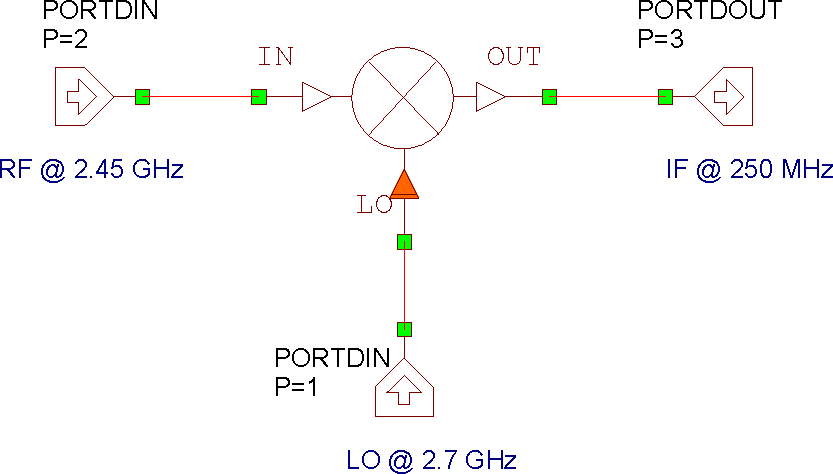
\includegraphics[scale=0.7]{MixerDiagram}
\caption{Schema del mixer.}
\label{fig:MixerDiagram}
\end{figure}

\noindent Il segnale a $f_\mathrm{RF}=2,45$ GHz (banda ISM 2.4 GHz) viene iniettato dalla porta RF per una sua mescolazione col segnale di battimento a $f_{LO}=2,7$ GHz immesso dalla porta LO generato dall'oscillatore locale. In uscita alla porta IF si ottengono i prodotti di miscelazione, tra i quali quello d'interesse a $f_\mathrm{IF}=250$ MHz ($f_\mathrm{IF}=f_\mathrm{LO}-f_\mathrm{RF}$). Il progetto del mixer si appoggia sul software Microwave Office dell'AWR mediante il quale � possibile valutarne prestazioni sfruttando il simulatore Harmonic Balance.

\section{Circuito del mixer a diodo singolo}

\par In figura \ref{fig:SingleDiodeMixer} viene illustrata l'implementazione circuitale del mixer a diodo singolo.

\begin{figure}[ht!]
\centering
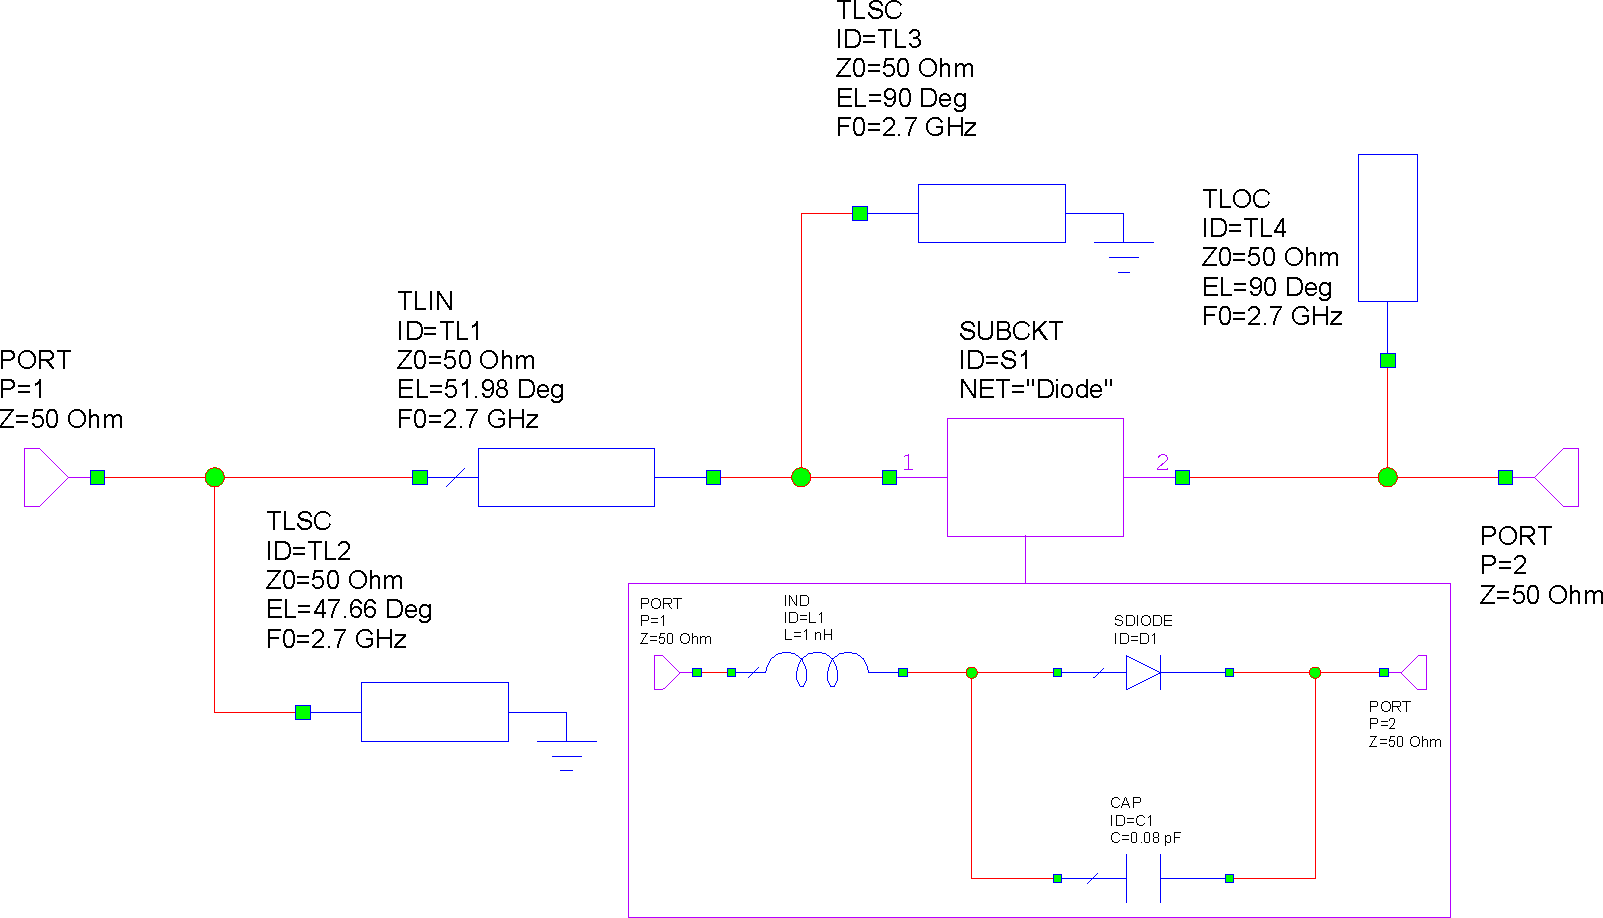
\includegraphics[scale=0.5]{SingleDiodeMixer}
\caption{Schematico del mixer a diodo singolo \textit{``Single Diode Mixer''}.}
\label{fig:SingleDiodeMixer}
\end{figure}

\noindent Il diodo, rappresentato dal sotto-circuito ``Diode''  � composto dal modello non lineare del diodo HSMS2850, i cui parametri sono deducibili dal datasheet fornito dal produttore \cite{HSMS2850DataSheet}, e dalle induttanza L1 e capacit� C1 parassite che rappresentano il comportamento elettrico del package SOT23.

\par La rete a L di adattamento � costituita dai tratti di linea TL1 e TL2 ideali, e l'adattamento viene eseguito in modo che l'impedenza differenziale del diodo pilotato dall'oscillatore locale a 2,7 GHz sia di 50 $\Omega$. In figura \ref{fig:LocalOscillator} � illustrato il circuito impiegato per l'adattamento dinamico. 
\begin{figure}[ht!]
\centering
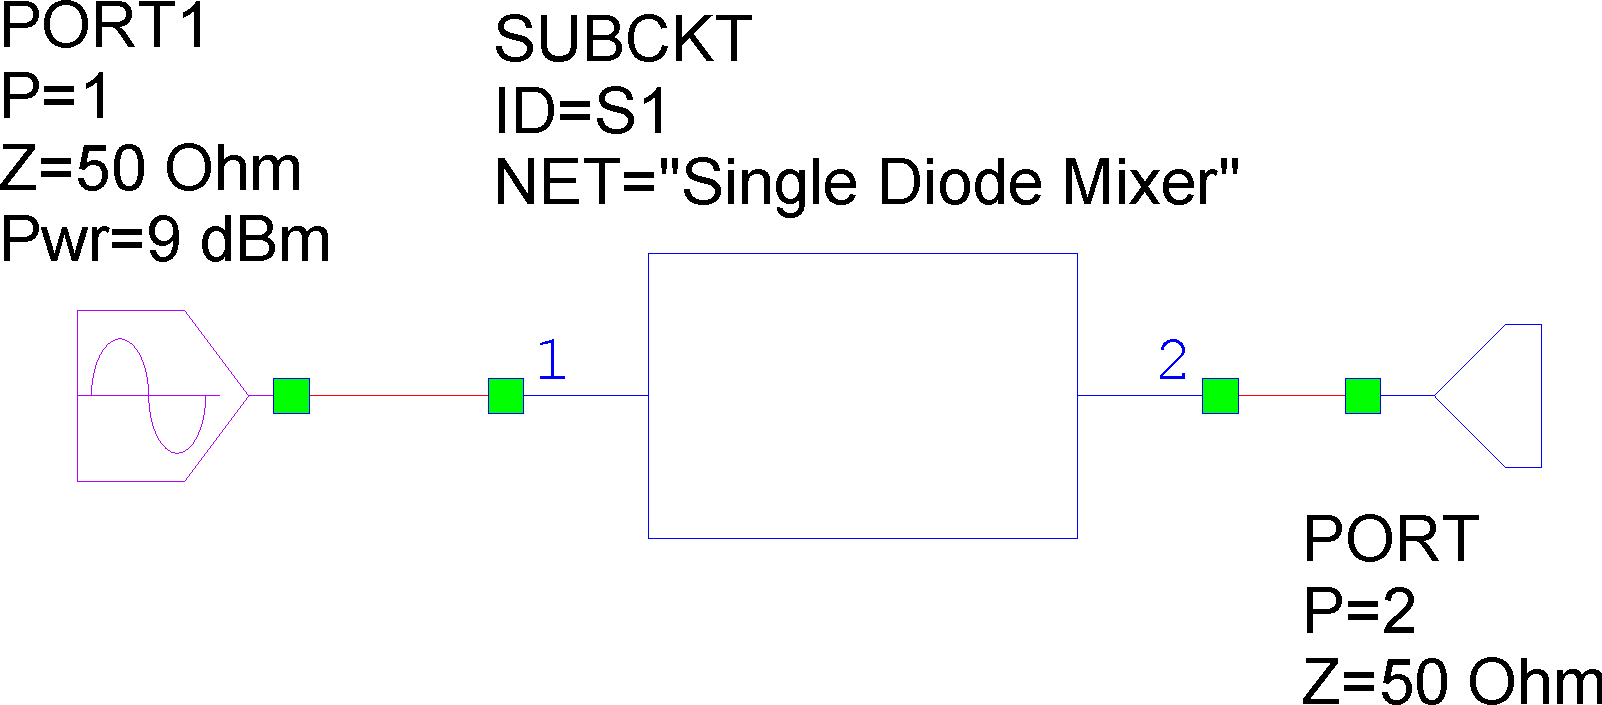
\includegraphics[scale=0.3]{LocalOscillator}
\caption{Circuito per l'adattamento dinamico a 2,7 GHz.}
\label{fig:LocalOscillator}
\end{figure}

\noindent L'adattamento assicura che la potenza generata dall'oscillatore locale giunga completamente al diodo massimizzando il meccanismo di \textit{switching} che sta alla base del mixer a diodo singolo.
\par Vi sono due ulteriori tratti di linea TL3 e TL4, rispettivamente all'anodo e al catodo del diodo. Questi stubs lunghi $\lambda/4$ a 2,7 GHz migliorano le prestazioni del mixer, richiudendo opportunamente la corrente erogata dall'oscillatore locale: il primo stub, in cortocircuito, f� si che venga visto in ingresso al diodo (anodo) un circuito aperto, mentre in uscita, lo stub in circuito aperto richiude in cortocircuito la corrente a 2,7 GHz fuoriuscente dal catodo, evitando il trasudamento o \textit{``feedthrough''} di tale componente spettrale all'uscita IF.
\par Prima di procedere con l'adattamento del diodo mediante lo strumento di \textit{tuning} sulle linee TL1 e TL2, � necessario modificare alcuni parametri del simulatore, ottimizzandolo per una simulazione non lineare tale quella richiesta dal progetto di un mixer. In figura \ref{fig:HBoptions} viene evidenziato il riquadro da modificare per ottimizzare la simulazione del mixer.
\begin{figure}[ht!]
\centering
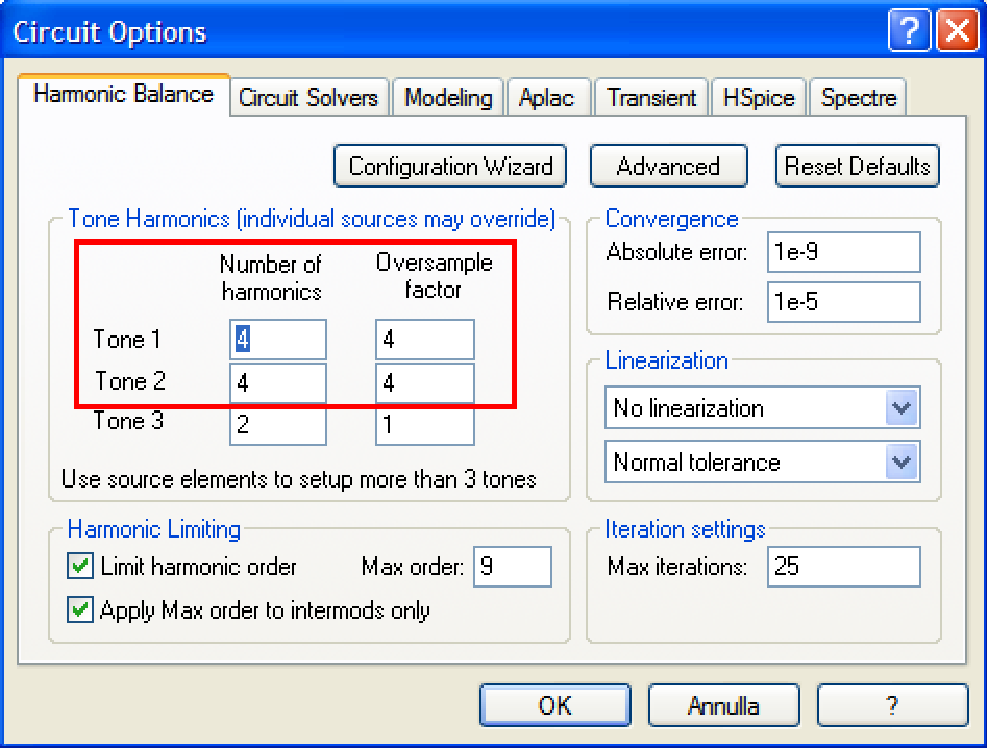
\includegraphics[scale=0.6]{HBoptions}
\caption{Finestra di impostazione del simulatore Harmonic Balance.}
\label{fig:HBoptions}
\end{figure} Sia per l'oscillatore locale (tono 1) che per il segnale RF (tono 2), il numero di armoniche da considerare viene portato a 4, e il fattore di sovracampionamento dei toni viene quadruplicato\footnote{Queste due operazioni si ripercuotono nell'accuratezza dei risultati ottenuti: la prima aumenta le componenti spettrali di influenza da considerare nella valutazione dei prodotti di miscelazione fino al 9� ordine (Figura \ref{fig:HBoptions}); la seconda garantisce, portando i dati campionati a 16 volte la frequenza di Nyquist, una maggior accuratezza nel matching dei risultati dal simulatore lineare e quello non lineare che compongono l'Harmonic Balance \cite{HBAgilent}.}. La frequenza di analisi viene impostata a 2,7 GHz nelle \textit{Project Options}.

\par Procediamo quindi con l'adattamento ``dinamico'' a 2,7 GHz, ossia individuando l'opportuna rete a L tale da adattare l'impedenza differenziale del diodo ai 50 $\Omega$ di impedenza di uscita dell'oscillatore locale. \`E proprio l'oscillatore locale, portando alternativamente in conduzione e in interdizione il diodo coi suoi 9 dBm, a generare un'impedenza differenziale $Z_{\textrm{D}} = {\left [\frac{ \partial{I_\textrm{D}}}{\partial{V_\textrm{D}}} \right ] }^{-1}$ di valore medio costante. In figura \ref{fig:DynamicMatching} viene illustrata sulla carta di Smith (normalizzata a $50 \Omega$) il parametro non lineare Gcomp, coefficiente di riflessione sul diodo valutato con l'Harmonic Balance alla frequenza di 2,7 GHz, ad adattamento compiuto.
\begin{figure}[ht!]
\centering
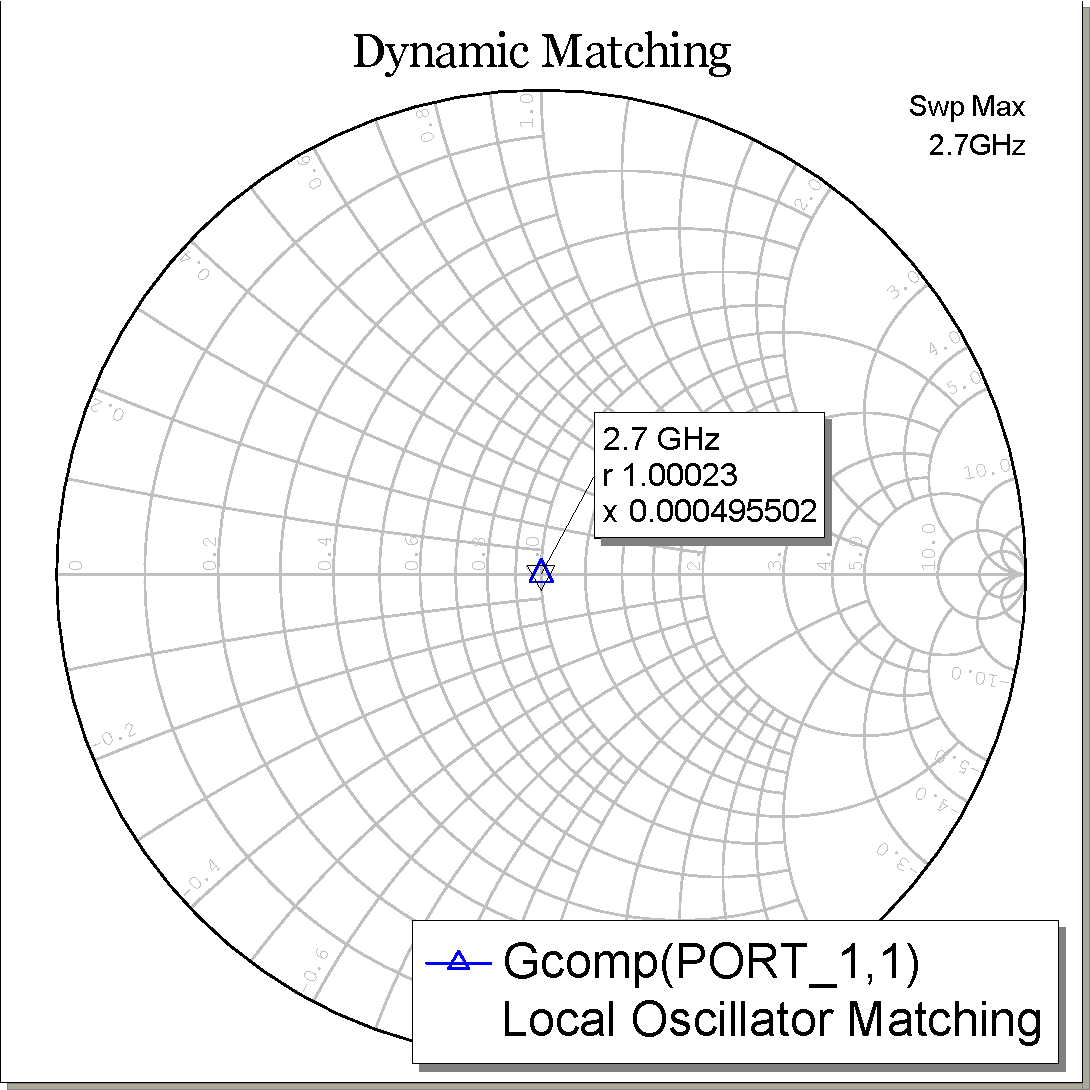
\includegraphics[scale=0.6]{DynamicMatching}
\caption{Adattamento dinamico sulla carta di Smith mediante il parametro Gcomp.}
\label{fig:DynamicMatching}
\end{figure}

\section{Prestazioni del mixer a diodo singolo}

\par Valutiamo adesso le prestazioni del mixer progettato. In una prima fase verr� simulato lo spettro in uscita alla porta IF del mixer a fronte di un segnale in ingresso RF a 2,45 GHz di -10 dBm. Viene quindi dedotta la perdita di conversione di tale mixer. In seguito verr� simulato lo spettro quando in ingresso vi siano due toni di -18 dBm, uno a 2,45 GHz, segnale desiderato, e uno a 2,5 GHz che rappresenti un segnale interferente giunto al mixer. Infine verr� valutata la dinamica d'ingresso del mixer in vista di ricavare il punto di compressione a -1 dB. Il segnale d'ingresso a 2,45 GHz verr� variato da una potenza di -23 dBm a 12 dBm.

\subsection{Prodotti di conversione}
\begin{figure}[ht!]
\centering
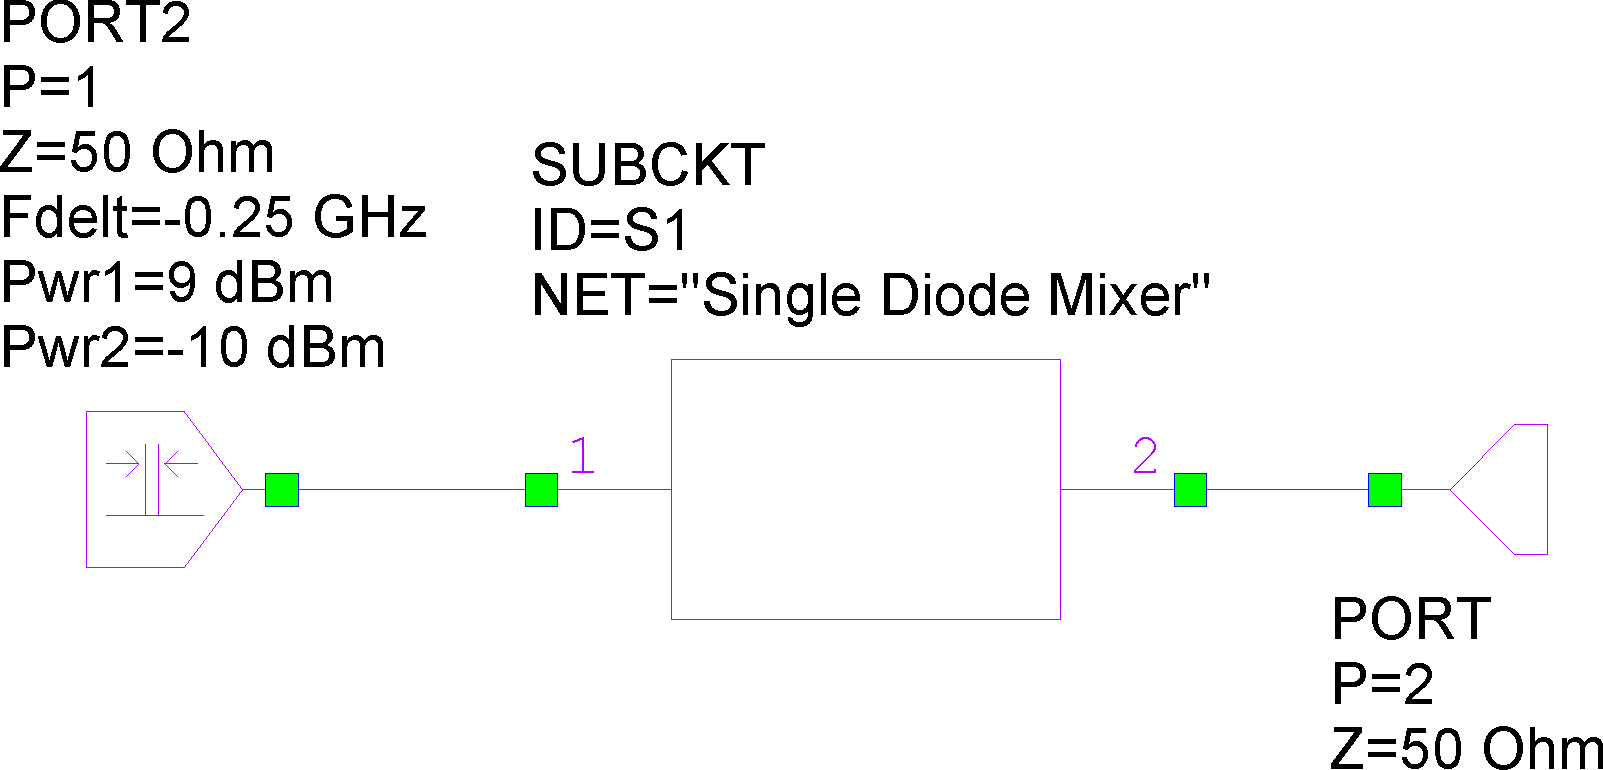
\includegraphics[scale=0.5]{SingleTone}
\caption{Circuito per la valutazione dei prodotti di miscelazione di un segnale RF di -10 dBm.}
\label{fig:SingleTone}
\end{figure}
\par Il circuito per la simulazione dello spettro in uscita dal mixer � quello illustrato in figura \ref{fig:SingleTone}. L'oscillatore locale (tono 1) eroga 9 dBm ed � adattato dinamicamente al diodo. Il segnale in ingresso RF (tono 2) � una riga spettrale di a 2,45 GHz di -10 dBm. Lo spettro di miscelazione � illustrato nella seguente figura \ref{fig:MixingProducts}.
\begin{figure}[ht!]
\centering
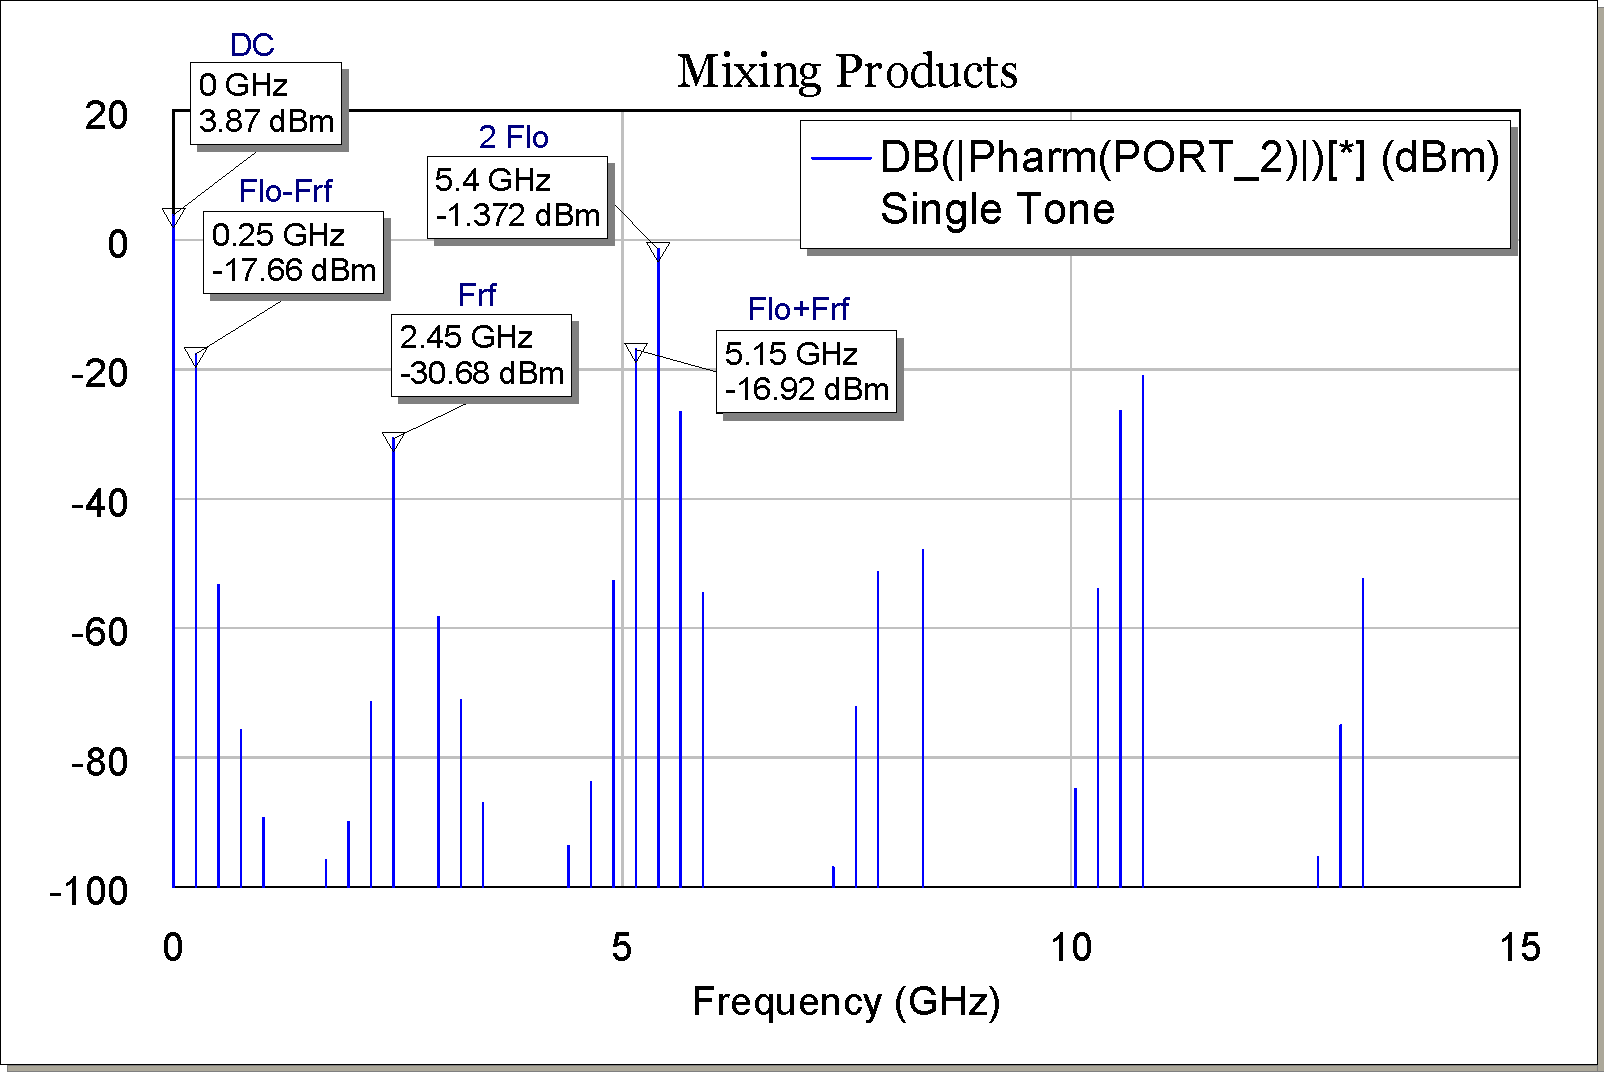
\includegraphics[scale=0.5]{MixingProducts}
\caption{Spettro IF a fronte di un ingresso RF a 2,45 GHz di -10 dBm.}
\label{fig:MixingProducts}
\end{figure} La componente spettrale a 250 MHz, prodotto di miscelazione del primo ordine ($f_\mathrm{IF} = f_\mathrm{LO}-f_\mathrm{RF}$) presenta un livello di potenza di -17,66 dBm. Deduciamo quindi che la perdita di conversione del mixer a diodo singolo progettato � di 7,66 dB. Questo � un risultato tipico per i mixer passivi \cite{CompleteWirelessDesign}. \`E presente una forte componente DC (3,87 dBm) legata alla struttura non bilanciata del mixer. Si notano inoltre il \textit{feedthrough} della componente a  $f_\mathrm{RF}$ e l'assenza di \textit{feedthrough} per quelle a $f_\mathrm{LO}$ e armoniche dispari, lo stub circuito aperto costituito dal tratto TL4 costringendo la porta IF a presentare un'impedenza molto bassa a tali frequenze. Come ce lo potevamo aspettare, la componente a frequenza somma $f_\mathrm{LO}+f_\mathrm{RF}$ � ampia circa quanto quella a $f_\mathrm{IF}$ (-16,92 dBm). 

\subsection{Prodotti di intermodulazione}

\par Vediamo adesso il comportamento del mixer in presenza di un interferente in banda alla frequenza ${f_\mathrm{RF}}_{interf}=2,5$ GHz, alla medesima potenza del segnale a $f_\mathrm{RF}=2,45$ GHz : -18 dBm. Questa � la tipica situazione che si ha quando avvengono contemporaneamente due conversazioni in un sistema di telecomunicazione FDM\footnote{Frequency Division Multiplexing.}: si ha \textit{crosstalk} se i sistemi ricetrasmittenti non sono sufficientemente selettivi in frequenza. In figura \ref{fig:TwoTones} � illustrato il circuito implementato per tale simulazione.
\begin{figure}[ht!]
\centering
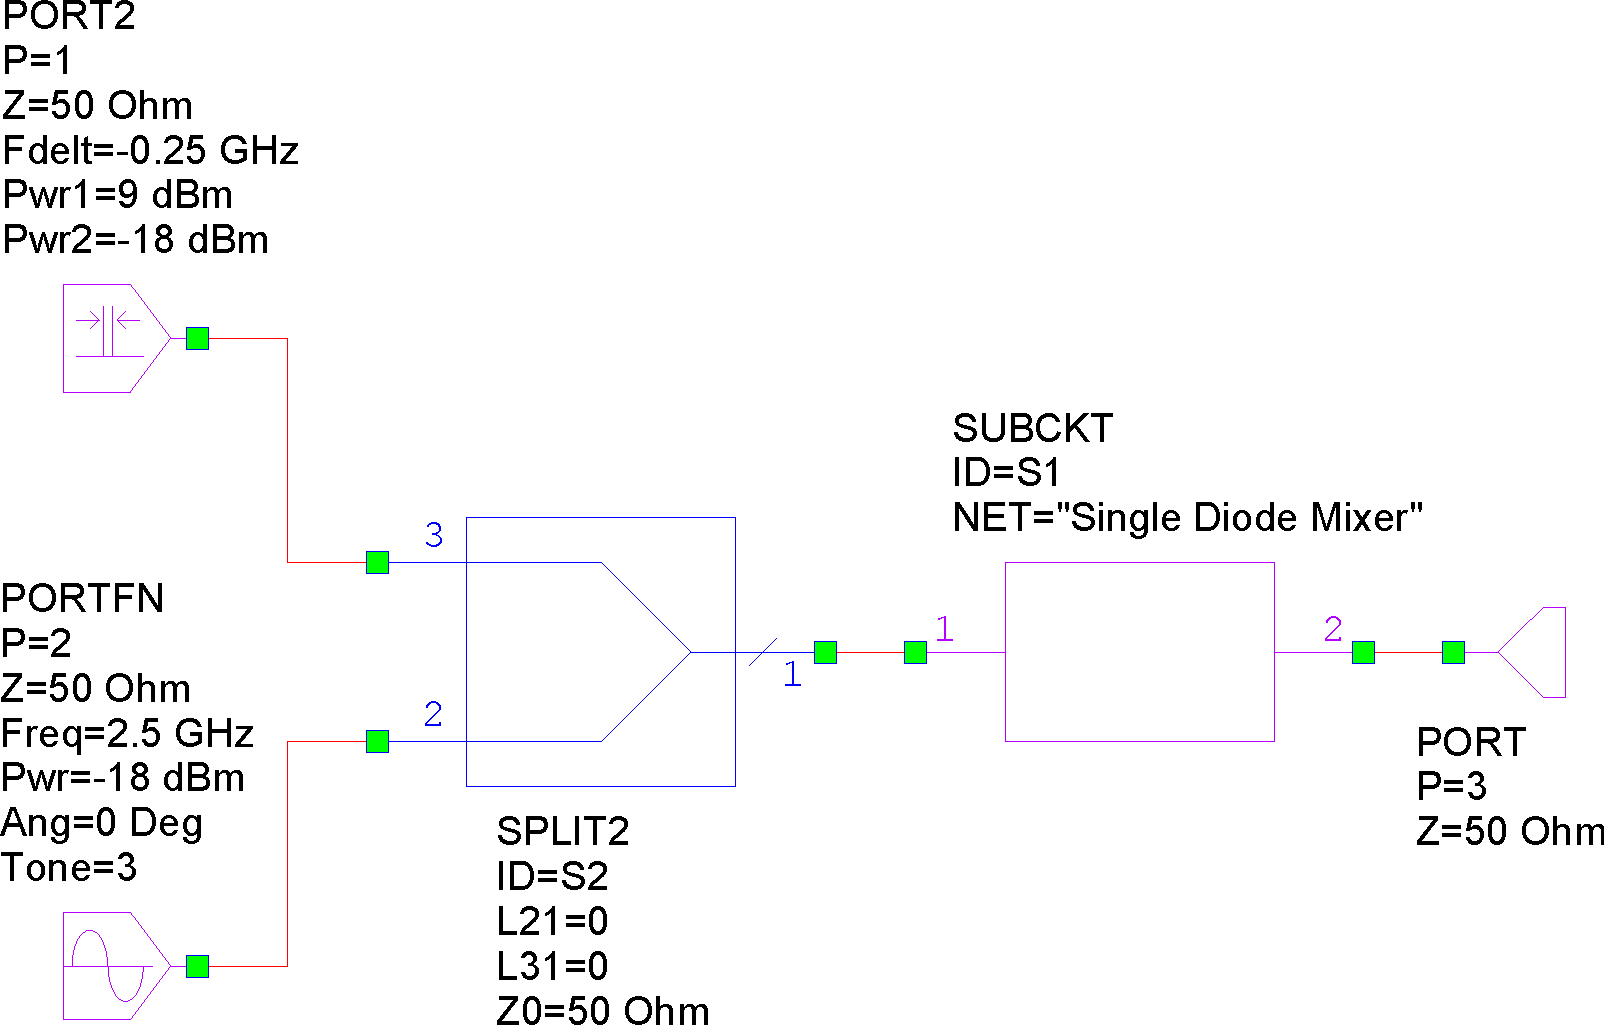
\includegraphics[scale=0.5]{TwoTones}
\caption{Circuito di valutazione delle componenti di intermodulazione a IF tra segnali di -18 dBm a $f_\mathrm{RF}$ e ${f_\mathrm{RF}}_{interf}$.}
\label{fig:TwoTones}
\end{figure} \`E stato utilizzato, per sommare i 3 toni a $f_\mathrm{RF}$, $f_\mathrm{LO}$ e ${f_\mathrm{RF}}_{interf}$ GHz, uno \textit{splitter} a 3 porte di uscita (dispositivo reciproco) idealmente privo di predite di inserzione tra la porta d'ingresso e quelle di uscita.
\par Per eseguire correttamente la simulazione, sono stati modificati i parametri relativi al tono 3 nelle opzioni dell'Harmonic Balance, portando a 4 sia il numero di armoniche da considerare che l'ordine di sovracampionamento.

\par In figura \ref{fig:IntermodulationProducts} viene illustrato lo spettro risultante alla porta IF.
\begin{figure}[ht!]
\centering
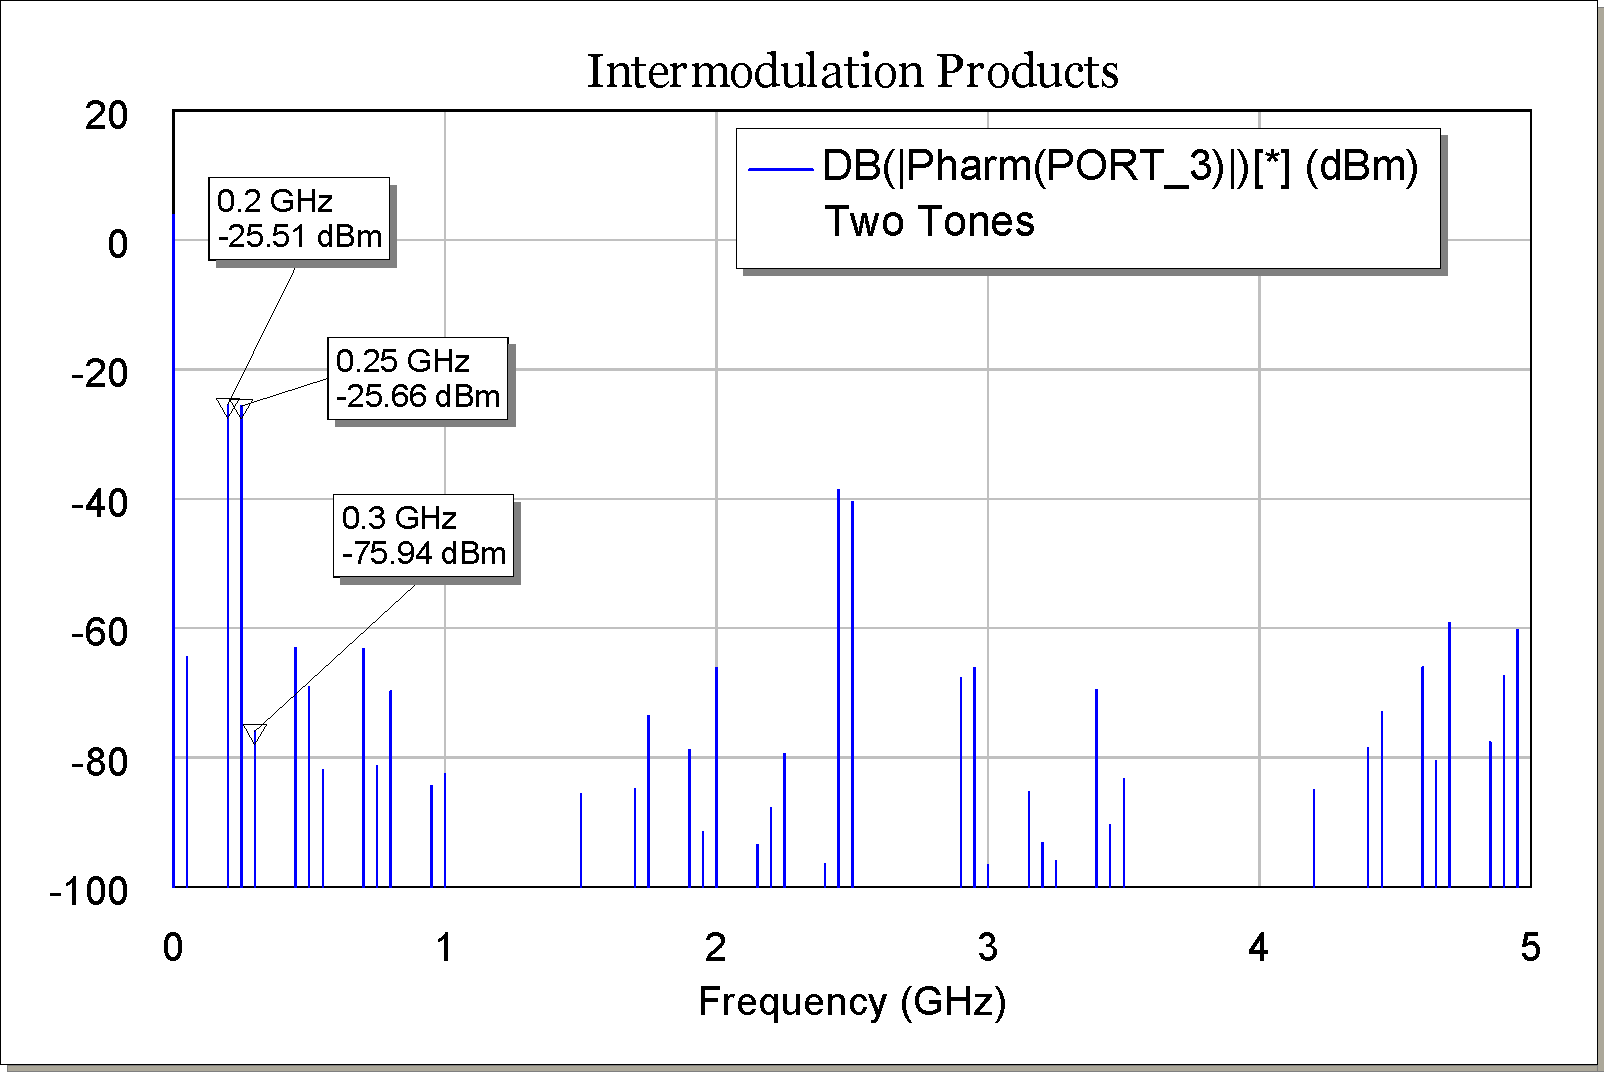
\includegraphics[scale=0.5]{IntermodulationProducts}
\caption{Spettro IF a fronte di un ingresso RF a 2,45 GHz di -18 dBm e di un disturbo a $f_\mathrm{RF_{interf}} = 2,5$ GHz dello stesso livello.}
\label{fig:IntermodulationProducts}
\end{figure} Sono evidenziate le componenti a 250 MHz, segnale d'interesse a frequenza intermedia, e quella a 200 MHz del disturbo \textit{down-converted} (canale adiacente a $f_\mathrm{RF_{interf}}$). Quest'ultimo sovrasta di poco pi� di 1 dB il segnale utile e i soli 50 MHz che li separa ne rendono critico l'isolamento. In effetti per attenuare il disturbo di soli 10 dB si dovrebbe ricorrere ad un filtro analogico del 5� ordine. 

\subsection{Dinamica d'ingresso e punto di compressione a -1dB}

\par Valutiamo infine la dinamica del mixer progettato, ricavando il \textit{range} di potenze entro il quale le perdite di conversione sono contenute 1 dB entro il valore nominale di 7,66 dB. In figura \ref{fig:1dBCompressionCircuit} � illustrato il circuito impiegato per la valutazione guadagno di conversione al variare della potenza in ingresso tra -23 e 12 dBm (\textit{sweep} della potenza del tono 2 con passi di 0,5 dB).

\begin{figure}[ht!]
\centering
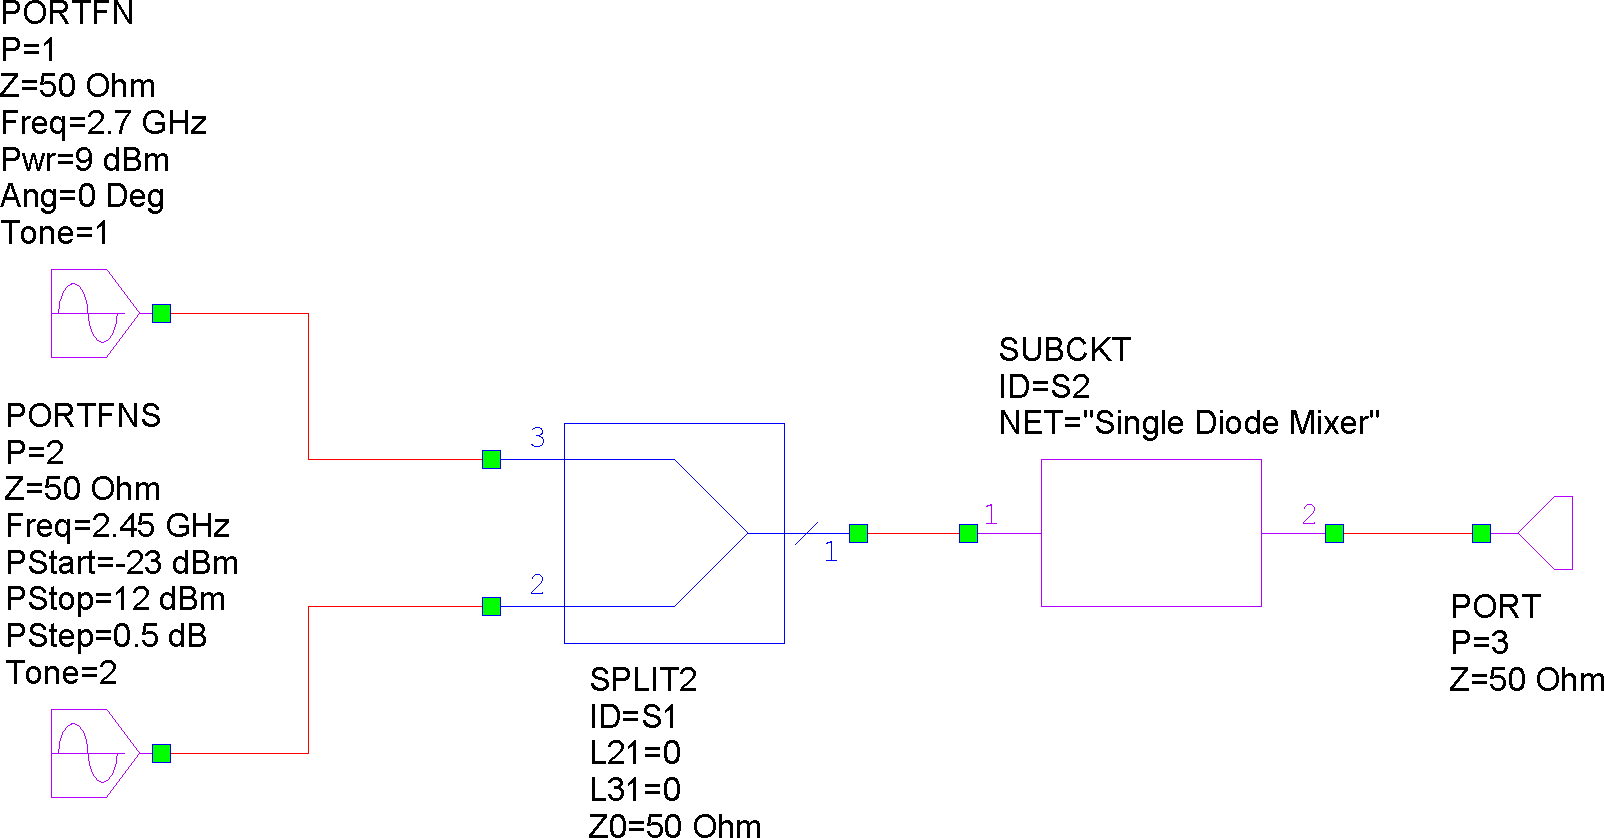
\includegraphics[scale=0.5]{1dBCompressionCircuit}
\caption{Circuito di simulazione della dinamica in ingresso e punto di compressione a -1 dB.}
\label{fig:1dBCompressionCircuit}
\end{figure}

\par In figura \ref{fig:1dBCompression} si vede l'andamento del guadagno di conversione, con la sua compressione ad una potenza in ingresso di 8,24 dBm.
\begin{figure}[ht!]
\centering
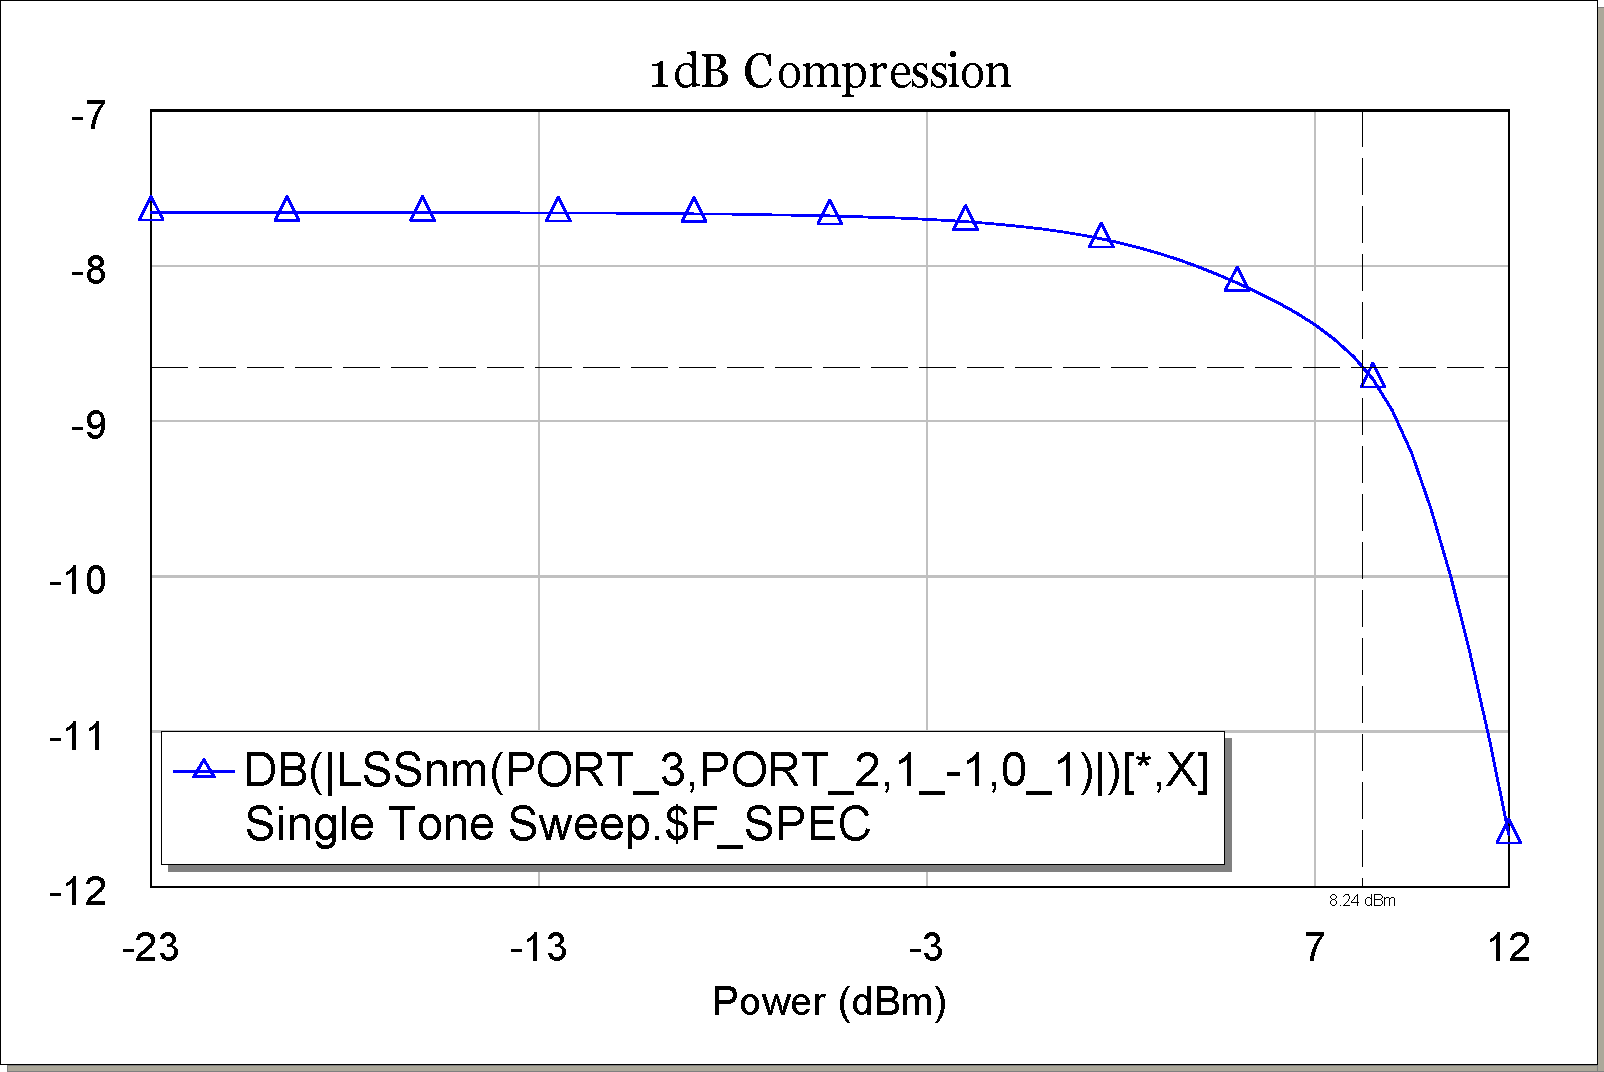
\includegraphics[scale=0.5]{1dBCompression}
\caption{Guadagno di conversione al variare della potenza RF in ingresso.}
\label{fig:1dBCompression}
\end{figure}

\section{Conclusione}

\begin{thebibliography}{9}

\bibitem{HSMS2850DataSheet} Agilent Tecnologies, Technical Data, \emph{HSMS-2850 Series}.

\bibitem{HBAgilent} Agilent Tecnologies, \emph{Guide to Harmonic Balance Simulation in ADS}, September 2004.

\bibitem{AWRUserGuide} Applied Wave Research, Inc., \emph{Microwave Office/Analog Office User Guide}, Version 6.51, January 2005.

\bibitem{CompleteWirelessDesign} C. W. Sayre, \emph{Complete Wireless Design}, MacGraw-Hill Telecom 2004.

\end{thebibliography}

\end{document}

\begin{figure}[ht!]
\begin{minipage}[b]{0.5\linewidth} % A minipage that covers half the page
\centering
\includegraphics[width=7cm]{GCompMeas}
\caption{Impostazione per l'adattamento non lineare del diodo.}
\label{fig:GCompMeas}
\end{minipage}
\begin{minipage}[b]{0.5\linewidth}
\centering
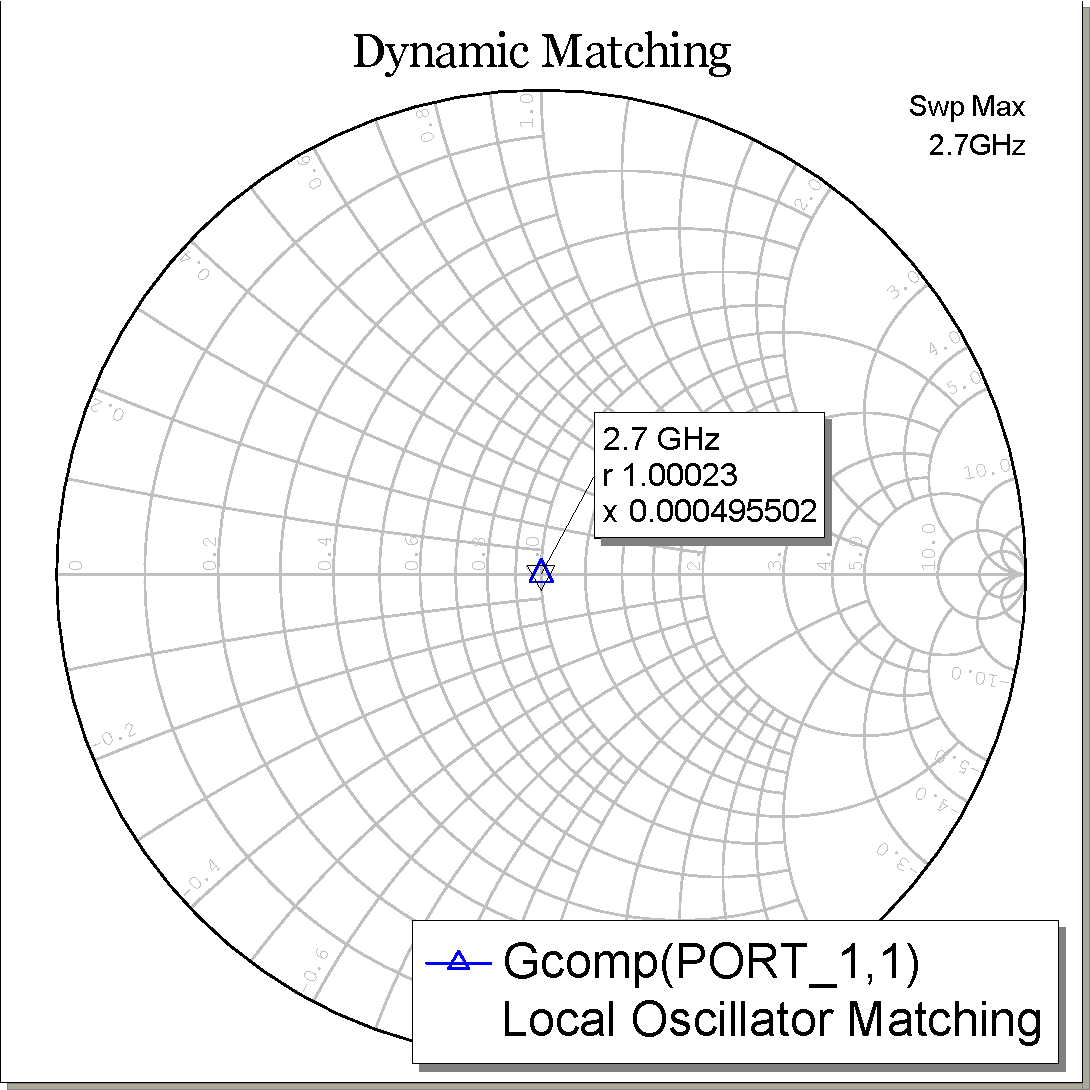
\includegraphics[width=7cm]{DynamicMatching}
\caption{Adattamento dinamico sulla carta di Smith mediante il parametro Gcomp.}
\label{fig:DynamicMatching}
\end{minipage}
\end{figure}
